\title{15-453 Final Report\\
       Neural Turing Machine}
\author{
        Eddy Yeo\\
                eyeo@andrew\\
            \and
        Yue Niu\\
                TODO\\
}
\date{\today}

\documentclass[12pt]{article}
\usepackage{amsmath, graphicx}
\graphicspath{{../images/copy_task/}}

\begin{document}
\maketitle

\begin{abstract}
We implement the Neural Turing Machine (Graves et al., 2014)\cite{DBLP:journals/corr/GravesWD14},
which is a neural network attached to an explicit memory store.
Given input and output sequences, it is able to learn small programs
that are remarkably similar to those that a human programmer would
write for a regular Turing Machine. Our implementation uses
TensorFlow, a software library for building neural networks
recently open sourced by Google.

\end{abstract}

\section{Introduction}

The Turing Machine is arguably the most well-known model of computation.
It is both sound and complete in an intuitive sense, meaning that it
is not able to do ``impossible things", and is able to do anything
that a reasonable model of computation could be expected to do.
It is known that there are other models of computation with equivalent
power -- Church's $\lambda$-calculus, $\mu$-recursive functions and
Herbrand-G\"odel computability being the few we learned in class. What
is perhaps the brilliance in the idea is the analogy to human computers.
A Turing Machine is a human with pen and paper, where the finite state
control is the mind of the human, the tape is the paper, and the pen is
the head. It will become clear in the subsequent sections why we
mention the pen as the head. This beautiful analogy has arisen once
again, but this time in the field now known as Deep Learning.

The recent increase in the availability of massive datasets and compute
power through the rise of large internet companies and Moore's Law have
revived a decades-old sub-field of computer science that has gone through
multiple rebrandings, the latest one being Deep Learning. These two
factors combined with various high profile performances of neural nets
(AlphaGo comes to mind) have resulted in much renewed interest. Two
innovations, explicit memory and attentional processes are found in
the Neural Turing Machine.

\paragraph{Outline}

The purpose of this paper is to set the context for our implementation.
Note that we assume some background knowledge of what a basic feedforward
neural network is, just to avoid having to describe everything from scratch.
The remainder of the paper is thus organized as follows.
Section~\ref{sequence} gives a brief overview of recurrent
neural networks and sequence learning.
In section~\ref{architecture} we explain the architecture of the Neural
Turing Machine. Section~\ref{tensorflow} talks a bit about the library
support that we have. In section~\ref{implementation} we
go into the technical details specific to our implementation.
Section~\ref{results} showcases the capabilities of our implementation.
We end off with our conclusion in section~\ref{conclusions}.

\section{Recurrent Neural Networks and Sequence Learning}\label{sequence}

Recurrent neural networks are neural networks that maintain state. They
do this by feeding one of their outputs back in as an input in the next time
step. They are known to be Turing-complete (Siegelmann and Sontag, 1992)\cite{Siegelmann:1992:CPN:130385.130432}
if the weights are rational, and are even capable of hypercomputation
if the weights are over the reals (Siegalmann and Sontag, 1994)\cite{SIEGELMANN1994331}.

They are very good at learning sequences especially if the lengths of
the sequences are not fixed. In a standard feedforward network, the
sequences would have to be encoded as a fixed-sized input, which is rather
limiting. However, if we model sequences as a series of inputs over time,
we can surpass this limitation. This is where recurrent neural networks come
in.

It turns out that learning sequences is hard when there are long-term
dependencies in the sequence. The basic construction of a recurrent
neural net, where the outputs of a unit are fed back into itself at the next
time step, does not work well because we have to encode this dependency
(over many time-steps) into a recurrent weight that will be applied at every
time-step. A successful solution to this problem are Long Short Term Memory
networks (LSTMs), that work by implementing gates for the recurrent 
links in the network, allowing the network to learn when to let information
pass through those parts. The Neural Turing Machine is a relatively new
but competitive design, especially for various kinds of tasks, as we
shall see.

\section{Architecture}\label{architecture}

The Neural Turing Machine is a neural network that is connected to a
memory store where it can store and read information from.
It is equipped with an addressing mechanism that allows it to focus its
attention on a particular spot in memory. This addressing mechanism
is analogous to the head of a turing machine. Its design is perhaps the
chief contribution of this paper. In a way, we might say that the Neural
Turing Machine is more about equipping the human with a pen,
rather than a writing surface, which is more trivial in comparison.

It is composed of three main components: the controller, the heads and 
the memory bank. The controller is just a regular neural network that will
both learn how to use the memory infrastructure via the heads that
it is provided with, and also predict the outputs
from the inputs and previous state. It can be a feedfoward network or
even an LSTM network. A feedforward network allows us to interprete
what the neural network is doing more easily, as any state it
stores has to be via one of the heads, while an LSTM network has
its own memory, which Graves likens to having registers in a computer to
augment its use of RAM.

The memory bank is just a two dimensional matrix that keeps state from
any output to it from one time step to the next, where it is used
as input (via a read head). Each column is a cell, and the number of
rows is the number of cells.

The head is a more
complicated addressing mechanism that chooses where in the memory matrix
to direct its output (i.e. store state). A key feature is that any writes
and reads are what Graves calls ``blurry", meaning that the head interacts
with the entire memory matrix at once, but is able to control the degree
of ``focus". This ensures that it remains differentiable, allowing it
to be trained with the regular gradient descent algorithms. A read at time
step $t$, which is used as one of the inputs along with the actual $t^{th}$
input, is just a weighted sum of the memory cells over all the rows:

$$
\mathbf{r}_t \leftarrow \sum_i w_t(i) \mathbf{M}_t(i)
$$

where $\sum_i w_t(i) = 1$ and $0 \le w_t(i) \le 1, \forall i$. The writing
mechanism follows a similar procedure, but with additional
details because it is allowed an additional erase step. The most critical part
of this whole architecture is for the network to be able to decide on the weight
vectors $\mathbf{w}_t$ intelligently. This brings us to the addressing mechanism.

\subsection{Addressing Mechanisms}

The addressing mechanism can be broadly divided into three main phases.
The first one is content-based focusing, the second is interpolating across
time steps, and the third is rotation. Each phase generates
a weight vector, with the latter two modifying the previous weight vectors generated
by the previous phase. The full details can be found in Grave's paper, but we
will go through them at a high level here.

The content-based mechanism allows the neural network to search for specific
content over the different cells. It does this by generating a key vector
$\mathbf{k}_t$, and then computing similarity scores over all the cells. It
then applies the softmax function to get the content weight vector. The
softmax function is also known as the normalized exponential, and is a 
good function to generate a probability distribution over different categories,
which is essentially what our weight vector is.

The interpolation phase allows the network to decide whether we want to use the weight
vector from the previous time step, or to use the new one freshly generated by our
content-based mechanism. This is essential to be able to iterate through tape cells,
as the location of our head depends on only its previous location and not its
content. The equation is as follows. Note that the interpolation factor $g_t$
lies between $0$ and $1$ and is generated by our controller. $\mathbf{w}^c_t$ is
the vector computed by our content-based mechanism.

$$
\mathbf{w}^g_t \leftarrow g_t\mathbf{w}^c_t + (1-g_t)\mathbf{w}_{t-1}.
$$

The last phase implements the rotation mechanism, which allows our network to
decide to shift the head left and right. It does this through circular convolution:

$$
\widetilde{w}_t(i) \leftarrow \sum_{j=0}^{N-1}w^g_t(j) s_t(i-j)
$$

The index of the shift vector $s_t$ is computed modulo the number of cells (rows)
in our memory matrix, $N$. The length of the shift vector is implicitly $N$, but
can be implemented with only the length of our shift width (the rest of the
values are implicitly zeroes). For example, if we
only allow shifts of $-1, 0, 1$, which has a shift width of $3$,
then the shift vector has length 3, and if
$i - (j - 1) \mod N$ is out of this range we just use $s_t(i-(j-1)) = 0$. Note
we have to use $j-1$ here instead of $j$ because our shift starts from $-1$. The
whole point of this operation is simply to rotate $\mathbf{w}^g_t$. The probability
distribution of the values in $s_t$ controls how much blurring occurs during the
rotation.

Note that throughout all these phases, care is taken to allow the neural net
to control the amount of blurring (or ``sharpening").
This is done by exponentiating and then
normalizing the weight vector between some of the phases, by a factor that is also
decided on by the controller. Once again, full details can be found in the original
paper.

\section{TensorFlow}\label{tensorflow}

Having described the basic network architecture, we now have to translate
these high-level descriptions into something that actually runs. There
are various considerations here. Firstly, we would like the code to 
run correctly. Neural networks involve a lot of floating point operations
over many time steps, where considerations of numerical stability
are paramount. Secondly, we want the code to run efficiently.
This means using matrix or at least vectorized operations in order to to
leverage highly optimized algorithms that have been developed over the years.
We also want the code to be somewhat hardware aware, to allow it to
exploit properties of the underlying computing system. The third consideration
is development time. Until now we have not really talked about the training
algorithms used, for example backpropagation. These algorithms involve knowing the
gradients of the operations we perform on the data, and ideally we do not want
to compute them by hand, especially if we are doing something new. Also,
we probably want our implementation to be able to run on GPU clusters, for instance,
without much modification. This is where the libraries come in.

The three big libraries in this area are Torch, Theano and Tensorflow. Torch is a framework
based on the Lua programming language and is actively maintained by Facebook AI. Theano
is a library based on Python and was originally developed by Yoshua Bengio's lab
at the Universit\'e de Montr\'eal. Tensorflow is also based on Python and is still
being actively developed by Google. We decided to use TensorFlow as we are comfortable
with Python and it seems to be well supported online by Google engineers
who are very responsive. The details can be found on the webpage and the white paper
\cite{tensorflow2015-whitepaper}. We will go over the basic details at a high level.

When we use Tensorflow, we are running python code that generates a computation
graph of operations. This is similar to the way futures work, in the sense
that the python code does not actually run any operations but rather
manipulates symbolic representations of these operations. After generating
our computation graph, we instruct the framework to actually run the computations.
This graph will be shipped off to a runtime written in a more efficient lower level
language and executed. The framework takes care of all the systems-level details.
Common operations and variants of the backpropagation algorithms are already implemented,
along with automatic gradient calculations. This allows us to worry only about the
high level details like neural network architecture, and greatly reduces our cognitive
load and development time. We should note that the operations in the computation graph
operate on tensors, which are $n$-dimentional arrays that represent our data as
it passes through our transformations.

\section{Implementation}\label{implementation}

We now go into the gory details of our implementation. The original paper left out
a surprising amount of detail, which might understandably have been
assumed to be background knowledge to those steeped in the field. Here are
some of them. We also talk about our design choices.

\subsection{Inputs, Outputs and Sequence-to-Sequence Training}

In terms of our experiment, we structured the training as follows. We
construct inputs-over-time/outputs-over-time pairs, where each inputs-over-time
is a sequence of inputs, the GO symbol, and then padding characters of the same length as the
expected output sequence. We need the padding characters as the neural network needs an input in order to
produce an output. (i.e. we need to cajole it to produce outputs after we are done
feeding our input sequence in). For some problems researchers feed in the output of the previous
timestep as the input of the current time step during the output phase,
instead of the padding character.
It was not clear to us which one was better, so
we chose the former due to simplicity of implementation. So for each inputs-over-time,
which comprise the input sequence, the GO symbol, and the padding symbols,
we will have an outputs-over-time of the same length.
Since we only care about the output sequence after the GO symbol,
our loss function is only computed on that portion.

\subsection{Read vs Write Heads}

It was not clear to us whether a head is both a read and write head, or if we
should have separate heads for both. We decided on separating the two types
because that makes our implementation more general.
Our current implementation assumes an equal number of read and write heads,
although it should be relatively simple to change this if necessary.

\subsection{Controller}

One of our primary goals was to see the neural net learn programs that are
similar to those a human would write for a turing machine. As such, we chose
to use a feedfoward controller because of its internal transparency. We want
to be able to track of all its state changes.

We used a single layer of $100$ hidden units, with the rectified linear unit (ReLU)
as their activation functions. This activation function has been shown to work
well despite its simplicitly, and also allows efficient training.
In his Deep Learning textbook (Bengio, 2016)\cite{Goodfellow-et-al-2016-Book}, Yoshua Bengio
mentions it as a good default for a hidden unit. Note that the sigmoid unit is now
commonly avoided as a hidden unit due to its gradient rapidly vanishing
as its output approaches either $0$ or $1$, making it less trainable by gradient
descent. It is still used though in output layers if the range needs to be between
$0$ and $1$.

The inputs for the current time step and read vectors (containing state read off
memory from the previous time step) are densely connected to the
hidden layer. The hidden layer is densely connected to the output layer, where the
predictions for the current time step are made, and the addressing parameter layer,
for internal use by the addressing mechanism.

For our addressing parameter layer, we used various activation functions depending
on what the parameter's value should fall between. Details can be found in
the original paper and the code.

We initialized most of our weights distributed uniformly between $(-0.1, 0.1)$.
It should be noted that a lot of these choices were experimentally determined -- we 
tried many of them and saw what worked.

\section{Results}\label{results}

\subsection{Copy Task}

Our first task was to train the Neural Turing Machine to reproduce a sequence
completely from memory. As described in the previous section, we first feed in
an input sequence, a special GO symbol and and then special padding symbols,
and we expect it to reproduce the input sequence after the GO symbol.
A simple feedforward network without any memory store will fail miserably
here as each padding symbol would just produce the same output.
We train it on sequences of random length between 1 to 5, where each character
in the sequence is a bit vector of width 3. Note that the GO symbol is just the
bit vector corresponding to $1$ and the padding symbol is just the bit vector
corresponding to $0$. We used the average cross-entropy
of the output sequence after the GO symbol as our loss. We gave the neural
network a memory matrix of size $50 \times 5$, meaning 50 cells, each cell being
able to store 5 bits. After 4100 iterations, at which the training loss was
consistently close to 0, we ran the resulting neural network on several test
sequences of varying length. We found that the neural network generalized
extremely well to sequences that were almost ten times the maximum length
it had seen during training. This is a result of having learned the correct
``program". Figure 1 shows the input and output vectors for a test sequence
of length $40$. The columns represent the bitvectors and the rows span
the sequence length. Each square is colored with a shade closer to red if the
bit is closer to 1, and closer to blue if the bit is closer to 0.
We see perfect recall the length of 40. When we get to 50, and we should
note that this is at the limit of the memory store that the neural network
is equipped with, we see from figure 2 that there are some minor corruptions
in the output.

\begin{figure}[h]
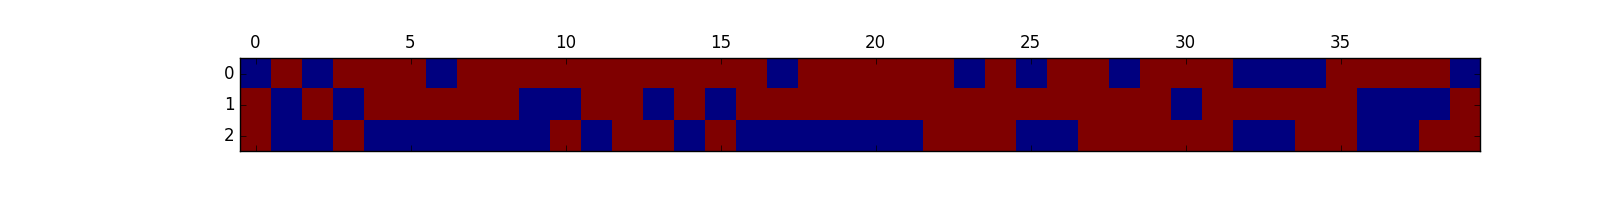
\includegraphics[width=\textwidth]{inputs40}
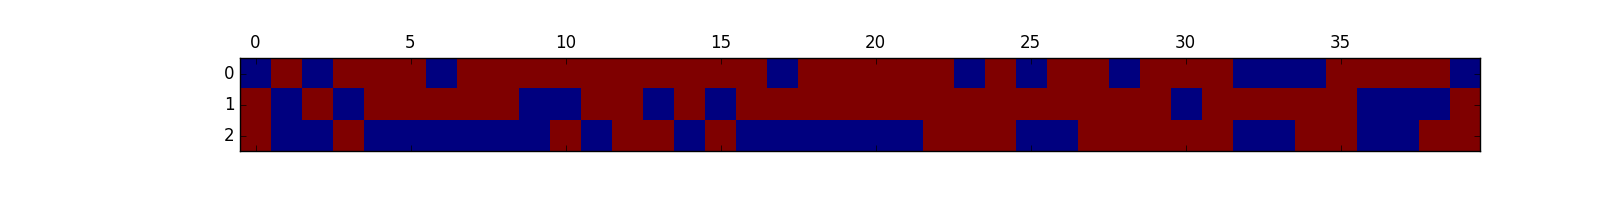
\includegraphics[width=\textwidth]{outputs40}
\caption{Sequence length of 40 (input on top)}
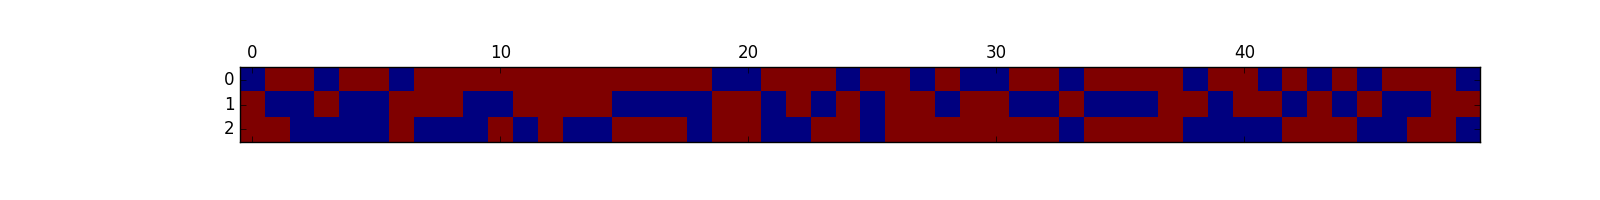
\includegraphics[width=\textwidth]{inputs50}
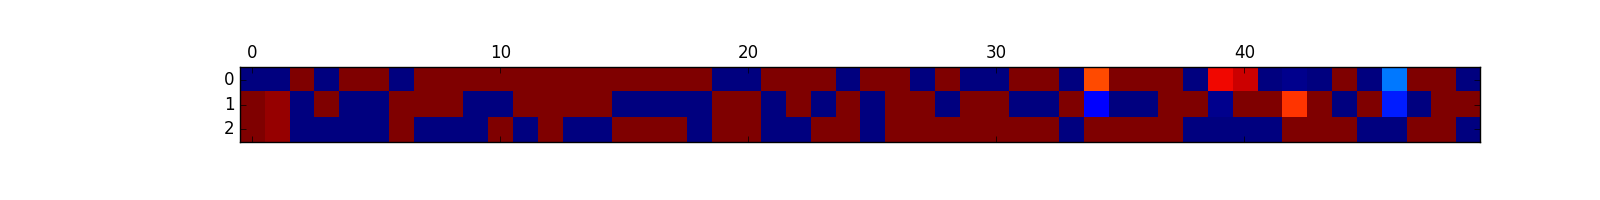
\includegraphics[width=\textwidth]{outputs50}
\caption{Sequence length of 50 (input on top)}
\end{figure}

Looking at the weight vectors at each time step, we are able to track
the head movements of the Neural Turing Machine. We see that the neural net has
implemented the ``obvious" program that solves
this problem. For each input, write it into the memory store and advance one cell.
When the
GO symbol is seen, start iterating over the saved input and output it.
Figure 3 below shows exactly this pattern. Each row represents the tape
at a specific time step, spanning over all time steps. The write head is seen to
be iterating until it has written 30 characters. Meanwhile the read head stays
put, and when 30 characters are seen it starts iterating. We chose this example
to show clearly that while the heads can approximate a turing machine head
pretty well when the neural net brings it into sharp focus, as in the read head's case,
the ``blurry" nature of the heads is still evident from the write head. We
see it dissipate into nothingness when it has done its job. Also note that
the head's rotation mechanism can wrap-around to the other end of the tape, 
as shown in the read head's movement.


\begin{figure}[h]
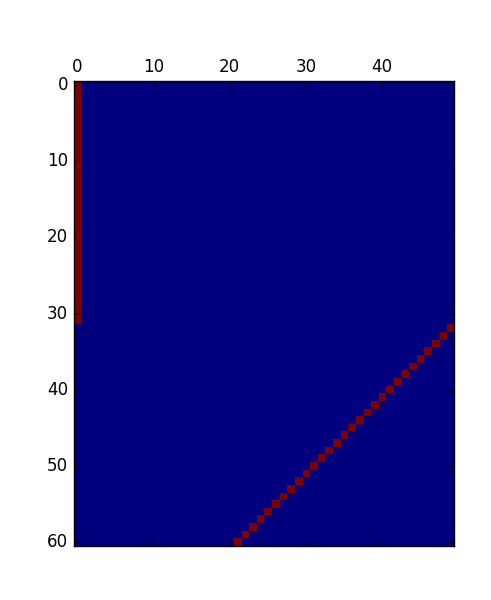
\includegraphics[width=0.5\textwidth]{read_head}
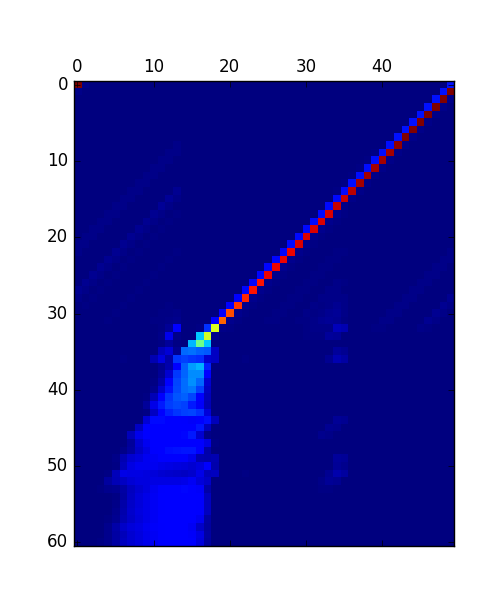
\includegraphics[width=0.5\textwidth]{write_head}
\caption{Head movements for sequence length of 30 (read head on left)}
\end{figure}

\subsection{Repeat Copy Task}

TODO

\section{Conclusions}\label{conclusions}

We have reproduced the published results on a smaller problem size for the
copy task. We see that the neural net has successfully learned how to
use its addressing mechanism and memory store very well, arguably to the
same level as a human programmer with a turing machine, at least for this
particular task. Learning to program also allowed it to generalize
well on sequences of far greater length.

TODO Kolmogorov-Complexity.

Accessibility. Support infrastructure and software. Multi-disciplinary.
Empirical field. A lot of intuition. Trial and error. Theory needed.

\bibliographystyle{abbrv}
\bibliography{report}

\end{document}
This is never printed
